\documentclass{amsart}

\usepackage{graphicx}
\usepackage{url}

\setlength{\parindent}{0pt}
\setlength{\parskip}{\baselineskip}

\DeclareMathOperator{\tr}{tr}

\begin{document}
\begin{center}
Science Atlantic Math Competition\\
Solutions
\end{center}

\textbf{Problem 1}\\
Show that the sum of five consecutive perfect squares is not itself a perfect square.

\textit{Solution}\\
Every set of five consecutive integers is of the form $\{n - 2, n - 1, n, n + 1, n + 2\}$.
The sum of the squares of these integers is $5(n^2 + 2)$.
If $5(n^2 + 2)$ is a perfect square, then $5 \mid (n^2 + 2)$.
But $-2$ is not a quadratic residue mod 5, so $5(n^2 + 2)$ is not a perfect square.

\textbf{Problem 2}\\
Let $m$ and $n$ be positive integers.
Suppose there are $m$ ants walking to the right and $n$ ants walking to the left along a line.
All ants walk at a constant speed and initially the right-walking ants are all to the left of the left-walking ants.

Whenever two ants collide, they immediately turn around and walk back in the opposite direction.
(Of course, if an ant turns around, it may then collide with the ant that was following it and turn around again, and so on).
Find (as a function of $m$ and $n$) the number of collisions that occur.

\textit{Solution}\\
The number of collisions is $mn$.

A collision does not change the numbers of ants moving left and right.
We may consider two ants reversing direction after a collision to instead have passed each other.
Each of the $m$ ants moving right must pass each of the $n$ ants moving left, so the total number of passings (or collisions) is $mn$.

\textbf{Problem 3}\\
Squares are erected outward on all four sides of a parallelogram.
Show that the centers of the squares themselves form a square.

\textit{Solution}\\
A parallelogram of width $w$ and height $h$ can be placed on the Cartesian plane with vertices at coordinates (counterclockwise)
\[ (0,0), (w, 0), (a + w, h), (a, h) \]
Now calculate that the centers of the erected squares (again counterclockwise) are
\[ \left( \frac{w}{2}, -\frac{w}{2} \right), \left( \frac{a + h + 2w}{2}, \frac{-a + h}{2} \right), \left( \frac{2a + w}{2}, \frac{2h + w}{2} \right), \left( \frac{a - h}{2}, \frac{a + h}{2} \right) \]
Finally using the Pythagorean theorem, the length of each side of the quadrilateral connecting these points is
\[ \frac{\sqrt{(a + h + w)^2 + (-a + h - w)^2}}{2} \]
and therefore the quadrilateral is a square.

\pagebreak

\textbf{Problem 4}\\
Let $\displaystyle y = x + \frac{x}{x + \frac{x}{x + \frac{x}{x + \cdots}}}$.
For what nonzero integer values of $x$ is $y$ also an integer?

\textit{Solution}\\
The only possible value of $x$ is $-4$.

The equation can be re-written as $y = x + \frac{x}{y}$, or $y^2 = (y + 1)x$.
Set $z = y + 1$; then $z^2 - 2z + 1 = zx$, implying that $z \mid 1$.
If $z = 1$ then $y = 0$ and $x = 0$, which is not permitted.
If $z = -1$ then $y = -2$ and $x = -4$, which is the only solution.

\pagebreak

\textbf{Problem 5}\\
Let $C$ be a unit cube.
Given any face $F$ of $C$, and any edge $e$ of $F$, let $V_{F, e}$ be the reflection of the center of $F$ in the edge $e$.
Let $V$ be the set of all points that can be obtained in this manner.
Sketch the convex polyhedron which has $V$ as its set of vertices, and describe it (with proof) in familiar terms.

\textit{Solution}\\
The polyhedron is a truncated octahedron with six square faces and eight regular hexagonal faces.

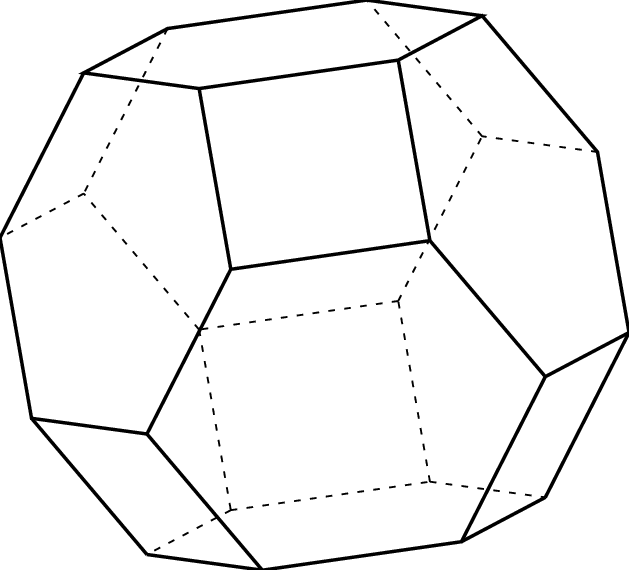
\includegraphics[width=10cm]{Images/Truncated-Octahedron}

\pagebreak

\textbf{Problem 6}\\
Determine all triples of rational numbers $(a, b, c)$ such that
\[ a^3 + 2b^3 + 4c^3 = 6abc \]

\textit{Solution}\\
The only solution is $(0, 0, 0)$.

Clearly $(0, 0, 0)$ is a solution.
Suppose towards contradiction there exists another rational solution $(a, b, c)$.

Let $q \in \mathbb{Q}$.
Multiplying both sides of the equation by $q^3$ and grouping, we have that
\[ (qa)^3 + 2(qb)^3 + 4(qc)^3 = 6(qa)(qb)(qc) \]
Therefore any rational multiple of a solution is a solution.
If $d_a, d_b, d_c$ are the least denominators of $a, b, c$, then $d_ad_bd_c(a, b, c)$ is an integer solution.
Finally, dividing an integer solution $(a, b, c)$ by $\gcd(a, b, c)$, there is an integer solution for which the three terms are coprime.

Without loss of generality let $(a, b, c)$ be an integer solution with $\gcd(a, b, c) = 1$.
Note that by the uniqueness of prime factorization, if a prime $p$ divides $n^3$ then $p$ divides $n$ for any $n \in \mathbb{Z}$.
Re-arrange the defining equation:
\[ a^3 = 2(3abc - b^3 - 2c^3) \]
Then $2 \mid a$ and we can write $a = 2a'$ for some integer $a'$.
\[ 2b^3 = 4(3a'bc - 2a'^3 - c^3) \]
As before, $2 \mid b$ and we can write $b = 2b'$ for some integer $b'$.
But now we have
\[ 4c^3 = 8(3a'b'c - a'^3 - 2b'^3) \]
and $2 \mid c$.
This is a contradiction because we assumed that $\gcd(a, b, c) = 1$.
Therefore there is no other rational solution $(a, b, c)$ and $(0, 0, 0)$ is the only one.

\pagebreak

\textbf{Problem 7}\\
An $n \times n$ matrix $A$ is said to have period $p$ if $p$ is the smallest positive integer such that $A^p = I_n$ (the $n \times n$ identity matrix).
For what $p$ is there a $2 \times 2$ matrix with integer elements that has period $p$?

\textit{Solution}\\
The possible values of $p$ are 1, 2, 3, 4, and 6.

Let $A = \begin{pmatrix} a & b \\ c & d \end{pmatrix}$ be a matrix with period $p$.

Recall that $\det(B)^n = \det(B^n)$ for all square matrices $B$ and positive integers $n$.
Therefore $\det(A)$ is a $p$-th root of unity, for the single eigenvalue of $I$ is 1.
But since $A$ is an integer matrix, $\det(A)$ must be an integer, either -1 or 1.

Recall that if $\lambda_1, \cdots, \lambda_m$ are the eigenvalues of $B$ for a square matrix $B$, then the eigenvalues of $B^n$ are $\lambda_1^n, \cdots, \lambda_m^n$.
Therefore the eigenvalues of $A$ are $p$-th roots of unity.

Calculate that the characteristic polynomial of $A$ is
\[ \lambda^2 - \tr(A) \lambda + \det(A) \]
Since the eigenvalues of $A$ are the roots of the characteristic polynomial of $A$, each eigenvalue $\lambda$ satisfies
\begin{align*}
\tr(A) \lambda &= \lambda^2 + \det(A) \\
\lvert \tr(A) \lambda \rvert &= \lvert \lambda^2 + \det(A) \rvert \\
\lvert \tr(A) \rvert &\leq \lvert \lambda^2 \rvert + \lvert \det(A) \rvert \\
\lvert \tr(A) \rvert &\leq 2
\end{align*}
Therefore the linear term of the characteristic polynomial is one of $0, \pm 1, \pm 2$ and the constant term is one of $\pm 1$.
There are ten polynomials which satisfy these conditions:
\begin{align*}
x^2 - 2x - 1 &= (x - (1 - \sqrt{2}))(x - (1 + \sqrt{2})) \\
x^2 - 2x + 1 &= (x - 1)(x - 1) \\
x^2 - x - 1 &= (x - \frac{1}{2}(1 - \sqrt{5}))(x - \frac{1}{2}(1 + \sqrt{5})) \\
x^2 - x + 1 &= (x - e^\frac{\pi i}{3})(x - e^\frac{5 \pi i}{3}) \\
x^2 - 1 &= (x - 1)(x + 1) \\
x^2 + 1 &= (x - i)(x + i) \\
x^2 + x - 1 &= (x - \frac{1}{2}(-1 - \sqrt{5}))(x - \frac{1}{2}(-1 + \sqrt{5})) \\
x^2 + x + 1 &= (x - e^\frac{2 \pi i}{3})(x - e^\frac{4 \pi i}{3}) \\
x^2 + 2x - 1 &= (x - (-1 - \sqrt{2}))(x - (-1 + \sqrt{2})) \\
x^2 + 2x + 1 &= (x + 1)(x - 1)
\end{align*}

\pagebreak

Picking from these roots only the roots of unity we find that the eigenvalues must be first, second, third, fourth, or sixth roots of unity.
Therefore the only possibilities for $p$ are 1, 2, 3, 4, 6.
It remains to give matrices which do indeed have this period:
\vspace{-14cm}
\begin{align*}
p &= 1 & \begin{pmatrix} 1 & 0 \\ 0 & 1 \end{pmatrix} \\
p &= 2 & \begin{pmatrix} -1 & 0 \\ 0 & -1 \end{pmatrix} \\
p &= 3 & \begin{pmatrix} -2 & -3 \\ 1 & 1 \end{pmatrix} \\
p &= 4 & \begin{pmatrix} 0 & 1 \\ -1 & 0 \end{pmatrix} \\
p &= 6 & \begin{pmatrix} 2 & 3 \\ -1 & -1 \end{pmatrix}
\end{align*}

\pagebreak

\textbf{Problem 8}\\
Determine the following quantity or prove that it does not exist:
\[ \lim_{n \to \infty} \sum_{j = 1}^n \frac{2^\frac{j}{n} - 2^\frac{j - 1}{n}}{2^\frac{j}{n} + 1} \]

\textit{Solution}\\
The series converges to $\ln(3) - \ln(2)$.

Note that given any $n$,
\[ [1, 2] = \bigcup_{j = 1}^n \left[ 2^\frac{j - 1}{n}, 2^\frac{j}{n} \right] \]
Also note that $2^\frac{j}{n} - 2^\frac{j - 1}{n}$ approaches 0 for all $1 \leq j \leq n$ as $n$ goes to infinity.
Therefore the sum $\displaystyle \sum_{j = 1}^n \frac{2^\frac{j}{n} - 2^\frac{j - 1}{n}}{2^\frac{j}{n} + 1}$ is a Riemann sum for $\displaystyle \frac{1}{1 + x}$ on the interval $[1, 2]$.
The limit as $n$ goes to infinity of the sum is then
\[ \int_1^2 \frac{\text{dx}}{1 + x} = \ln(3) - \ln(2) \]
\end{document}